\chapter{Grundlagen}
\label{sec:grundlagen}
\section{Zustandsraumdarstellung}
\label{subsec:zustandsraumdarstellung}
Der Zustandsraum ist der Raum, in dem das System durch die Zustandsgrößen aufgespannt wird. Es ermöglicht einen Einblick in das Innere des Systems, indem die im System gespeicherten Energien (Energiemomentaufnahme) erfasst werden und als Matrizen und Vektoren dargestellt werden.
Darstellung im Zeitbereich, d.h. wir gehen von Differentialgleichung des Systems aus. Für die Zustandsraumdarstellung zweiter Ordnung müssen wir die eine Differentialgleichung zweiter Ordnung in zwei Differentialgleichungen erster Ordnung transformieren.
Wir müssen immer eine DG höherer Ordnung erst in mehrere DG erster Ordnung umformen, denn: Bei der Darstellung des Systems spendieren wir pro DG einen Integrator und dieser Integrator kann nur genau einmal integrieren, also nur eine DG erster Ordnung modellieren.
D.h. wir haben nach der Transformation nur DG erster Ordnung.
Dies geschieht indem wir Zustandsvariablen einführen, die einen n-dimensionalen Vektorraum aufspannen, in der dann Zustandstrajektorien gezeichnet werden können. Energiespeicher sind z.B. Masse und Feder. 
\begin{flushleft}
Zustandsgleichung:
$  \vec{\dot{x}} = A\vec{x}+B\vec{u} = $
$
\begin{pmatrix}
a_1 & a_2 & a_3 & a_4 \\
b_1 & b_2 & b_3 & b_4 \\
c_1 & c_2 & c_3 & c_4 \\
d_1 & d_2 & d_3 & d_4
\end{pmatrix}
$ 
\end{flushleft}
\begin{flushleft}
Ausgangsgleichung:
$  \vec{y} = c\vec{x}+d\vec{u} $
\end{flushleft}
Dabei sind: A die Systemmatrix, B die Eingangsmatrix, C die Ausgangsmatrix, D die Durchgangsmatrix. \\
A gibt den Zusammenhang an zwischen Zustandsgrößen $\vec{x}$ und Änderungsgeschwindigkeiten der Zustandsgrößen $\vec{\dot{x}}$. \\
B stellt Zusammenhang her zwischen Eingangsgrößen und Änderungsgeschwindigkeiten der Zustandsgrößen $\vec{\dot{x}}$. \\
C stellt Zusammenhang her zwischen Zustandsgrößen $\vec{x}$ und Ausgangsgrößen $\vec{y}$. \\
D beschreibt, wie die Eingangsgrößen $\vec{u}$ direkt auf die Ausgangsgrößen $\vec{y}$ wirken (Nur bei direkter Verbindung). \\

\section{inverse und direkte Kinematik}
\label{subsec:inverse und direkte Kinematik}
Die direkte Kinematik berechnet in der Robotik aus den Gelenkwinkeln eines Roboters die Pose (Position und Orientierung) und ist damit das Gegenteil der inversen Kinematik, die wiederum aus der Pose die Gelenkwinkel bestimmen kann. Abbildung 2.1 zeigt den Zusammenhang.
\begin{figure}[htb]
  \centering  
  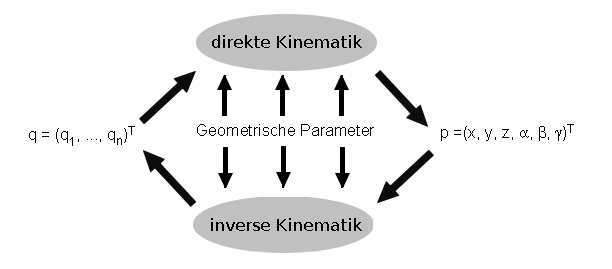
\includegraphics[scale=2.5]{img/Roboterkinematik.png}
  \caption{inverse und direkte Kinematik}
  \label{fig:inverse und direkte Kinematik}
\end{figure}
Bei unserer Arbeit betrachten wir keinen Roboter, sondern ein Fahrzeug, weswegen in unserem Modell aus der Geschwindigkeit des gesamten fahrenden Systems in die Winkel- und die Lineargeschwindigkeit (direkte Kinematik) und zurück (inverse Kinematik) umgerechnet werden kann. Aber dazu in Kapitel 4 genaueres.

